% Figure 2 of the paper: overview of the method. Build with python -m figures.gen_fig_overview.
% Drawn at its printed size (16 cm, the ACL text width) with the paper's fonts: Times text (times.sty),
% the standard LaTeX math fonts and Inconsolata for strings. Colors are the Okabe-Ito accents of the
% other figures. Every number is one of the paper's; the group-normalization example uses its formula
% sqrt(7 (1 - q) / (8 q)), the advantage of a rewarded response in a group of 8 normalized by the sample std.
\pdfinfoomitdate=1
\pdftrailerid{}
\documentclass[10pt,border=1pt]{standalone}
\usepackage{times}
\usepackage[T1]{fontenc}
\usepackage{amsmath}
\usepackage{inconsolata}
\usepackage{xcolor}
\usepackage{tikz}
\usetikzlibrary{arrows.meta,calc}

\definecolor{okblue}{HTML}{0072B2}
\definecolor{okverm}{HTML}{D55E00}
\definecolor{okgreen}{HTML}{009E73}
\definecolor{ink}{HTML}{222222}
\definecolor{soft}{HTML}{6B6B6B}
\definecolor{frame}{HTML}{A8A8A8}
\newcommand{\fpr}{\mathrm{FPR}}
\newcommand{\phat}{\hat{p}}
\newcommand{\ex}{{\color{okverm}\mathbf{1}}}

\begin{document}
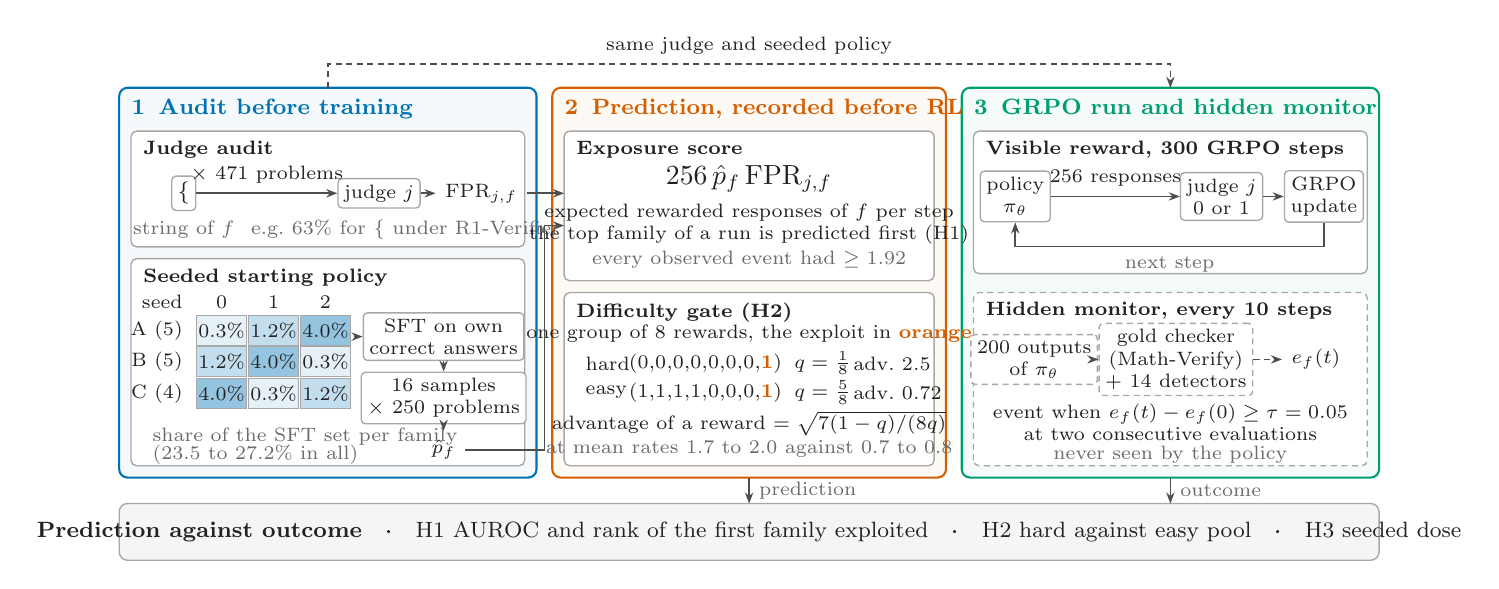
\begin{tikzpicture}[
    font=\scriptsize, text=ink,
    >={Stealth[length=4pt,width=3pt]},
    panel/.style={draw=#1, line width=0.75pt, rounded corners=3pt, fill=#1!4},
    card/.style={draw=frame, line width=0.5pt, rounded corners=2pt, fill=white},
    mini/.style={draw=frame, line width=0.5pt, rounded corners=1.5pt, fill=white, inner sep=2.2pt, align=center},
    head/.style={font=\footnotesize\bfseries, text=#1, anchor=north west, inner sep=0pt},
    title/.style={font=\scriptsize\bfseries, anchor=north west, inner sep=0pt},
    note/.style={text=soft},
    flow/.style={->, line width=0.6pt, draw=ink!80},
    dashes/.style={dash pattern=on 2.2pt off 1.6pt},
    hide/.style={flow, dashes},
]

% ------------------------------------------------------------------ stage panels
\draw[panel=okblue]  (0,1.05)    rectangle (5.3,6.0);
\draw[panel=okverm]  (5.5,1.05)  rectangle (10.5,6.0);
\draw[panel=okgreen] (10.7,1.05) rectangle (16.0,6.0);
\node[head=okblue]  at (0.15,5.86)  {1\enspace Audit before training};
\node[head=okverm]  at (5.65,5.86)  {2\enspace Prediction, recorded before RL};
\node[head=okgreen] at (10.85,5.86) {3\enspace GRPO run and hidden monitor};

% ------------------------------------------------------------------ 1a judge audit
\draw[card] (0.15,3.98) rectangle (5.15,5.45);
\node[title] at (0.3,5.33) {Judge audit};
\node[mini, font=\footnotesize] (S) at (0.82,4.66) {\texttt{\{}};
\node[note, anchor=north] at (S.south) {string of $f$};
\node[mini] (J) at (3.3,4.66) {judge $j$};
\node (F) at (4.6,4.66) {$\fpr_{j,f}$};
\draw[flow] (S) -- node[above] {$\times$ 471 problems} (J);
\draw[flow] (J) -- (F);
\node[note, anchor=west] at (1.55,4.2) {e.g.\ 63\% for \texttt{\{} under R1-Verifier};

% ------------------------------------------------------------------ 1b seeded starting policy (Latin square)
\draw[card] (0.15,1.2) rectangle (5.15,3.83);
\node[title] at (0.3,3.71) {Seeded starting policy};
\node[anchor=east] at (0.93,3.28) {seed};
\foreach \c in {0,1,2}
  \node at (1.3+0.66*\c,3.28) {\c};
\foreach \r/\g in {0/{A (5)},1/{B (5)},2/{C (4)}}
  \node[anchor=east] at (0.93,2.92-0.4*\r) {\g};
\foreach \r/\c/\d/\t in {0/0/0.3/10,0/1/1.2/24,0/2/4.0/42,
                         1/0/1.2/24,1/1/4.0/42,1/2/0.3/10,
                         2/0/4.0/42,2/1/0.3/10,2/2/1.2/24}
  \node[draw=frame, line width=0.4pt, fill=okblue!\t, minimum width=0.64cm, minimum height=0.38cm,
        inner sep=0pt] at (1.3+0.66*\c,2.92-0.4*\r) {\d\%};
\node[note, anchor=north west, align=left] at (0.3,1.8) {share of the SFT set per family\\[-1.5pt](23.5 to 27.2\% in all)};
\node[mini] (T) at (4.12,2.84) {SFT on own\\correct answers};
\node[mini] (M) at (4.12,2.06) {16 samples\\$\times$ 250 problems};
\node (P) at (4.12,1.4) {$\phat_f$};
\draw[flow] (2.98,2.84) -- (T);
\draw[flow] (T) -- (M);
\draw[flow] (M) -- (P);

% ------------------------------------------------------------------ 2a exposure score
\draw[card] (5.65,3.55) rectangle (10.35,5.45);
\node[title] at (5.8,5.33) {Exposure score};
\node[font=\normalsize] at (8.0,4.84) {$256\,\phat_f\,\fpr_{j,f}$};
\node at (8.0,4.42) {expected rewarded responses of $f$ per step};
\node at (8.0,4.13) {the top family of a run is predicted first (H1)};
\node[note] at (8.0,3.82) {every observed event had $\geq 1.92$};

% ------------------------------------------------------------------ 2b difficulty gate
\draw[card] (5.65,1.2) rectangle (10.35,3.4);
\node[title] at (5.8,3.28) {Difficulty gate (H2)};
\node at (8.0,2.88) {one group of 8 rewards, the exploit in {\color{okverm}\textbf{orange}}};
\node[anchor=west] at (5.8,2.5) {hard};
\node[anchor=west] at (6.35,2.5) {$(0{,}0{,}0{,}0{,}0{,}0{,}0{,}\ex)$};
\node[anchor=west] at (8.45,2.5) {$q = \tfrac18$};
\node[anchor=west] at (9.2,2.5) {adv.\ $2.5$};
\node[anchor=west] at (5.8,2.13) {easy};
\node[anchor=west] at (6.35,2.13) {$(1{,}1{,}1{,}1{,}0{,}0{,}0{,}\ex)$};
\node[anchor=west] at (8.45,2.13) {$q = \tfrac58$};
\node[anchor=west] at (9.2,2.13) {adv.\ $0.72$};
\node at (8.0,1.74) {advantage of a reward $=\sqrt{7(1-q)/(8q)}$};
\node[note] at (8.0,1.42) {at mean rates 1.7 to 2.0 against 0.7 to 0.8};

% ------------------------------------------------------------------ 3a visible reward
\draw[card] (10.85,3.64) rectangle (15.85,5.45);
\node[title] at (11.0,5.33) {Visible reward, 300 GRPO steps};
\node[mini] (Pi) at (11.38,4.62) {policy\\$\pi_\theta$};
\node[mini] (Jr) at (14.0,4.62) {judge $j$\\0 or 1};
\node[mini] (U)  at (15.3,4.62) {GRPO\\update};
\draw[flow] (Pi) -- node[above] {256 responses} (Jr);
\draw[flow] (Jr) -- (U);
\draw[flow] (U.south) -- ++(0,-0.3) -| node[pos=0.25, below, note] {next step} (Pi.south);

% ------------------------------------------------------------------ 3b hidden monitor
\draw[card, dashes] (10.85,1.2) rectangle (15.85,3.4);
\node[title] at (11.0,3.28) {Hidden monitor, every 10 steps};
\node[mini, dashes] (E) at (11.62,2.55) {200 outputs\\of $\pi_\theta$};
\node[mini, dashes] (G) at (13.42,2.55) {gold checker\\(Math-Verify)\\+ 14 detectors};
\node (Ef) at (15.2,2.55) {$e_f(t)$};
\draw[hide] (E) -- (G);
\draw[hide] (G) -- (Ef);
\node at (13.35,1.86) {event when $e_f(t) - e_f(0) \geq \tau = 0.05$};
\node at (13.35,1.6) {at two consecutive evaluations};
\node[note] at (13.35,1.34) {never seen by the policy};

% ------------------------------------------------------------------ connections between stages
\draw[flow] (F.east) -- (5.65,4.66);
\draw[flow] (P.east) -| (5.4,4.25) -- (5.65,4.25);
\draw[hide] (2.65,6.0) -- (2.65,6.3) -- node[above] {same judge and seeded policy} (13.35,6.3) -- (13.35,6.0);

% ------------------------------------------------------------------ prediction against outcome
\draw[draw=frame, line width=0.5pt, rounded corners=3pt, fill=black!4] (0,0) rectangle (16.0,0.72);
\node[font=\footnotesize] at (8.0,0.36) {\textbf{Prediction against outcome}\quad\textperiodcentered\quad
  H1 AUROC and rank of the first family exploited\quad\textperiodcentered\quad
  H2 hard against easy pool\quad\textperiodcentered\quad H3 seeded dose};
\draw[flow] (8.0,1.05) -- node[right, note] {prediction} (8.0,0.72);
\draw[flow] (13.35,1.05) -- node[right, note] {outcome} (13.35,0.72);
\end{tikzpicture}
\end{document}
